\documentclass[aspectratio=169]{beamer}
\usepackage{standalone}

\usepackage{stmaryrd}
\usepackage{listings}
\usepackage{bussproofs}

\usepackage[hyperref=auto,style=alphabetic,backend=bibtex]{biblatex}
\addbibresource{kwarcpubs.bib}
\addbibresource{extpubs.bib}
\addbibresource{extcrossrefs.bib}
\usepackage{appendixnumberbeamer}
\usepackage{tikz}
\usepackage{tikz-qtree}
\usetikzlibrary{arrows.meta}
\usetikzlibrary{mmt}
\usetikzlibrary{docicon}

\usetheme{Pittsburgh}
\setbeamertemplate{footline}[frame number]
\setbeamertemplate{navigation symbols}{}
\usecolortheme{beaver}
\setbeamertemplate{frametitle}[default][left]
% \setbeamersize{text margin left=3em}

\usepackage{utils/colors}
\usepackage[forbeamer]{utils/basic}
\usepackage{utils/operators}
\usepackage{utils/mylstmisc}
\usepackage{utils/lstmmt}

\lstset{basicstyle=\ttfamily}
\lstset{commentstyle=\itshape\color{commentfont}}

\title{GLIF: A declarative framework for Montague-style natural language semantics}

\author{Jan Frederik Schaefer}
\institute{FAU Erlangen-N\"urnberg/KWARC}
\date{\textbf{Seminar: Computing Meaning}\\Hildesheim\\July 21, 2022}

\begin{document}
\frame\titlepage


\begin{frame}
    \frametitle{whoami}
    \begin{itemize}
        \item PhD student in the KWARC group (Erlangen)
            \com{Knowledge representation}
        \item We teach a lecture in \emph{logic-based natural language semantics}
        \item Wanted more hands-on experience
        \item $\leadsto$ new framework: GLIF\com{Grammar, Logic, Inference}
    \end{itemize}
\end{frame}

% \begin{frame}
    \frametitle{Natural Language Understanding (NLU)}
    \textbf{My definition:}\\
    NLU means translating natural language into a formal semantic representation.

    \vspace{2em}
    \makebox[9cm]{\str{How many people live in Slovakia?}} $\leadsto\;\;$ \str{5.458 million}

    \vspace{1em}
    \makebox[9cm]{\str{Do more people live in Slovakia than in Thailand?}} $\leadsto\;\;$ ???

    \vspace{2em}
    \centering
    \begin{tikzpicture}
        \node (nbnd) at (1.2,0.7) {useless};
        \node (bnd) at (3.5,0.7) {\begin{tabular}{c}also in-\\teresting\end{tabular}};
        \node (bd) at (3.5,2.0) {AI-complete?};
        \node (nbd) at (1.2,2.0) {\begin{tabular}{c}this\\work\end{tabular}};
        \draw[->,very thick] (-0.3,0) -- (5,0);
        \draw[->,very thick] (0,-0.3) -- (0,2.7);
        \node at (4.0, -0.3) {\itshape breadth};
        \node[rotate=90] at (-0.3,1.8) {\itshape depth};
    \end{tikzpicture}
\end{frame}


\begin{frame}
    \frametitle{Method of Fragments}
    \only<1-2>{
        \centering
        \only<1>{\def\fraglevel{0}}
        \only<2>{\def\fraglevel{1}}
        \includestandalone{fig/montague-fragments}

        \begin{minipage}[t][2cm]{\textwidth}\vspace{1em}
            How do we get from messy language to formal logic?\\[0.5em]
            \emph{Montague}~\cite{Montague:efl70}: Look at a ``nice'' subset
            and map into logic.
        \end{minipage}
    }

    \only<3>{
        \centering
        \def\fraglevel{1}
        \includestandalone{fig/montague-fragments}
        
        \begin{minipage}[t][2cm]{0.6\textwidth}\vspace{1em}
            \str{Ahmed paints and Berta is quiet.}\\[0.5em]
            \str{Ahmed doesn't paint.}
        \end{minipage}\hfill
        \begin{minipage}[t][2cm]{0.39\textwidth}\vspace{1em}
            $p(a) \wedge q(b)$\\[0.5em]
            $\neg p(a)$
        \end{minipage}
    }

    \only<4>{
        \centering
        \def\fraglevel{2}
        \includestandalone{fig/montague-fragments}
        
        \begin{minipage}[t][2cm]{0.6\textwidth}\vspace{1em}
            \str{Every student paints and is quiet.}\\[0.5em]
            \str{Nobody paints.}
        \end{minipage}\hfill
        \begin{minipage}[t][2cm]{0.39\textwidth}\vspace{1em}
            $\forall x.s(x) \Rightarrow (p(x) \wedge q(x))$\\[0.5em]
            $\neg \exists x.p(x)$
        \end{minipage}
    }

    \only<5>{
        \centering
        \def\fraglevel{3}
        \includestandalone{fig/montague-fragments}

        \begin{minipage}[t][2cm]{0.6\textwidth}\vspace{1em}
            \str{Ahmed isn't allowed to paint.}\\[0.5em]
            \str{Ahmed and Berta must paint.}
        \end{minipage}\hfill
        \begin{minipage}[t][2cm]{0.39\textwidth}\vspace{1em}
            $\neg\lozenge p(a)$\\[0.5em]
            $(\square p(a)) \wedge \square p(b)$
        \end{minipage}
    }
\end{frame}


\begin{frame}
    \frametitle{Method of Fragments}
    {\color{hlfont}Hand-waving} is problematic:

    \hspace{2em}\str{Ahmed paints. He is quiet.}
    {$\quad\stackrel{?}{\leadsto}\quad$ \color{logicfont} $p(a)\wedge q(a)$}

    \vspace{1.2em}
    {\color{hlfont}Montague}: Specify
    \begin{itemize}
        \item grammar,\com{fixes NL subset}
        \item target logic,
        \item semantics construction.\com{maps parse trees to logic}
    \end{itemize}

    {
        \centering
        \vspace{0.3em}
        {\itshape\footnotesize Example from~\cite{Montague:tptoqi73}}

        \vspace{0.2em}\fbox{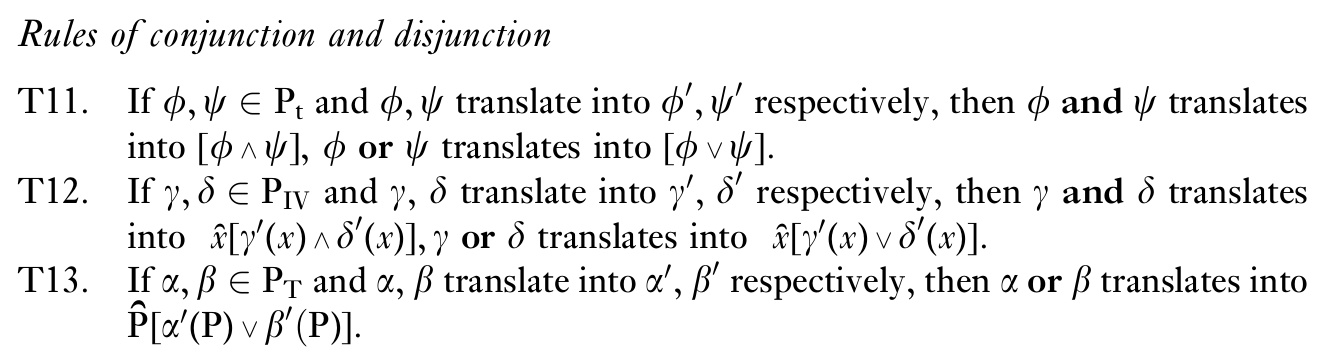
\includegraphics[trim=0 0 0 80,clip,width=0.7\textwidth]{fig/montague-tptoqioe.png}}

        \vspace{1.2em}
        Claim: That doesn't scale well $\leadsto$ \textbf{We need {\color{hlfont}prototyping}!}
    }

    % \newcommand\VP{\text{\upshape\tiny VP}}
    % \hspace{2em}$\llbracket\text{\strplain{$P_{\VP}$ and $Q_{\VP}$}}\rrbracket_{\VP} = \lambda x. \llbracket\text{\strplain{$P_{\VP}$}}\rrbracket(x) \wedge \llbracket\text{\strplain{$Q_{\VP}$}}\rrbracket(x)$
\end{frame}


\begin{frame}[fragile]
    \frametitle{NLU Prototyping}
    \begin{lstlisting}[mathescape,keywords=translate,keywordstyle=\bf,
                       morestring={[d]"}, stringstyle=\it,showstringspaces=false]
> translate "Every student paints and is quiet."
$\forall$x.s(x)$\Rightarrow$(p(x)$\wedge$q(x))
    \end{lstlisting}
    \vspace{1em}
    \begin{itemize}
        \item Traditionally done in Prolog/Haskell
        \begin{itemize}
            \item[$\raa$] requires a lot of work
        \end{itemize}
            \item A dedicated framework might be better
        \begin{itemize}
            \item[$\raa$] only partial solutions exist
        \end{itemize}
        \item Can we combine existing partial solutions? % \com{Research Question}
        \begin{itemize}
            \item[$\leadsto$] GLIF
        \end{itemize}
    \end{itemize}
\end{frame}



{
    \enablepart{showjupyter}
    \disablepart{showepistemicexample}
    \disablepart{mentionprovergen}
    \provideenablepart{showspa}
\providedisablepart{showepistemicexample}
\provideenablepart{showjupyter}

\begin{frame}
    \frametitle{Components of GLIF: GF}
    \enablepart{hlgf}
    \includestandalone[width=\textwidth]{fig/glif-architecture}
\end{frame}

\begin{frame}[fragile]
    \frametitle{Components of GLIF: Grammatical Framework \cite{GF:on}}
    \begin{itemize}
        \item Specialized for developing natural language grammars
        \item Separates abstract and concrete syntax\par
            \quad\lstinline[language=GF]|sentence : NP -> VP -> S;               --abstract|\par
            \quad\lstinline[language=GF]|sentence np vp = np.s ++ vp.s!np.n;   --concrete|
        \item Abstract syntax based on LF
        \item Comes with large library \com{$\ge 36$ languages}
    \end{itemize}

    \vspace{2em}
    \hspace{2.5em}\begin{tikzpicture}
        \node(eng) at (-2,0.7) {\str{Ahmed paints}};
        \node(ger) at (-2,-0.7) {\str{Ahmed zeichnet}};
        \node(ast) at (4,0) {
                    \color{logicfont!50!nlfont}
                    \resizebox{2.cm}{!}{\tikzset{edge from parent/.append style={very thick}}
                        \Tree [ .\texttt{sentence} \texttt{ahmed} \texttt{paint} ]
                    }
                };
        \draw[<->, thick] (eng) to node[above,rotate=-9]{Eng. concr. syn.} (ast);
        \draw[<->, thick] (ger) to node[below,rotate=9]{Ger. concr. syn.} (ast);
    \end{tikzpicture}
\end{frame}

\begin{frame}
    \frametitle{Components of GLIF: MMT}
    \enablepart{hlmmt}
    \includestandalone[width=\textwidth]{fig/glif-architecture}
\end{frame}

\begin{frame}[fragile]
    \frametitle{Components of GLIF: MMT}
    \lstset{frame=single}
    \begin{itemize}   
        \item Modular logic development and knowledge representation
        \item Not specialized in one logical framework \com{we use LF}
        \item We will use MMT to:
        \begin{itemize}
            \item { \only<2>{\bf\color{hlfont}} represent abstract syntax }
            \item { \only<3>{\bf\color{hlfont}} specify target logic and discourse domain theory}
            \item { \only<4>{\bf\color{hlfont}} specify semantics construction}
        \end{itemize}
    \end{itemize}
    \lstset{basicstyle=\footnotesize\ttfamily}
    
    \vspace{1em}
    \begin{minipage}[t][4cm]{\textwidth}
        \centering
        \only<2>{% Used in slides/glif-components.tex
% Has to be in separate file...
\begin{minipage}[t]{0.35\textwidth}
    \parbox[t][1em][t]{\textwidth}{\centering\bf GF}\par
    \begin{lstlisting}[language=GF,linewidth=\textwidth]
cat
  NP; VP; S;
fun
  sentence :
    NP -> VP -> S;
    \end{lstlisting}
\end{minipage}
\begin{minipage}[t]{0.1\textwidth}\vskip3em \centering\LARGE$\mapsto$\end{minipage}
\begin{minipage}[t]{0.3\textwidth}
    \parbox[t][1em][t]{\textwidth}{\centering\bf MMT}\par
    \begin{lstlisting}[language=MMT,linewidth=\textwidth]
NP : type
VP : type
S  : type
sentence :
  NP \raa VP \raa S \end{lstlisting}
\end{minipage}
}
        \only<3>{% Used in slides/glif-components.tex
% Has to be in separate file...
\begin{minipage}[t]{0.45\textwidth}
    \parbox[t][1em][t]{\textwidth}{\centering\bf Logic}\par
    \begin{lstlisting}[language=MMT,linewidth=\textwidth]
o : type //propositions
\neg : o \raa o
\wedge : o \raa o \raa o
\vee : o \raa o \raa o

\iota : type //individuals
\forall : (\iota \raa o) \raa o
\exists : (\iota \raa o) \raa o \end{lstlisting}
\end{minipage}\hskip2em
\begin{minipage}[t]{0.3\textwidth}
    \parbox[t][1em][t]{\textwidth}{\centering\bf Domain Theory}\par
    \begin{lstlisting}[language=MMT,linewidth=\textwidth]
paint : \iota \raa o
quiet : \iota \raa o
ahmed : \iota
berta : \iota \end{lstlisting}

    \footnotesize
    \vspace{1.5em}
    \hskip-1em
    idea:
    $\forall f$
    or $\forall \lambda x.f(x)$\par
    \hskip-1em instead of $\forall x.f(x)$
\end{minipage}
}
        \only<4>{\textbf{Semantics Construction}

\ifpart{narrowslides}{\small}{}
\textit{map symbols in abstract syntax to terms in logic/domain theory}

\vspace{0.5em}
\begin{minipage}[t]{0.4\textwidth}
\parbox[t][1em][t]{\textwidth}{\centering Simple setting}\par
\ifpart{switchtomathexample}{
    \lstinputlisting[language=MMT]{slides/misc/snippets/s000.txt}
}{
    \lstinputlisting[language=MMT]{slides/misc/snippets/s001.txt}
}
\end{minipage}
\hspace{1em}
\begin{minipage}[t]{0.5\textwidth}
\parbox[t][1em][t]{\textwidth}{\centering More advanced}\par
\ifpart{switchtomathexample}{
    \lstinputlisting[language=MMT]{slides/misc/snippets/s002.txt}
}{
    \lstinputlisting[language=MMT]{slides/misc/snippets/s003.txt}
}
\end{minipage}
}
    \end{minipage}
\end{frame}

\begin{frame}[fragile]
    \frametitle{Example: Parsing + Semantics Construction}
    {\centering\str{Ahmed and Berta paint}\par}\vspace{1em}
    \hspace{0.49\textwidth}$\downarrow_{\text{parsing}}$\par\vspace{1em}
    {\centering\color{logicfont!50!nlfont} sentence (andNP ahmed berta) paint\par}\vspace{1em}
    \hspace{0.49\textwidth}$\downarrow_{\text{semantics construction}}$\par\vspace{1em}
    {\centering\begin{adjustbox}{}\color{logicfont}\footnotesize\lstinline[language=MMT]|(\lambdan.\lambdav.n v) ((\lambdaa.\lambdab.\lambdap.a p \wedge b p) (\lambdap.p ahmed) (\lambdap.p berta)) paint|\end{adjustbox}\par}\vspace{1em}
    \hspace{0.49\textwidth}$\downarrow_{\text{$\beta$-reduction}}$\par\vspace{1em}
    {\centering\color{logicfont}\small\begin{adjustbox}{}\lstinline[language=MMT]|paint ahmed \wedge paint berta|\end{adjustbox}\par}
\end{frame}

\begin{frame}
    \frametitle{Components of GLIF: ELPI}
    \enablepart{hlelpi}
    \includestandalone[width=\textwidth]{fig/glif-architecture}
\end{frame}

\provideenablepart{mentionprovergen}
\begin{frame}[fragile]
    \frametitle{Components of GLIF: ELPI}
    \begin{itemize}
        \item Implementation and extension of $\lambda$Prolog\com{$\approx$ Prolog + HOAS}
        \item MMT can generate logic signatures
        \ifpart{mentionprovergen}{
            \item First experiments with prover generation
        }{}
        \item Generic inference/reasoning step after semantics construction
        \item Goal: Use it for semantic/pragmatic analysis
    \end{itemize}
    \lstset{basicstyle=\footnotesize\ttfamily}

    \vspace{1em}
    \centering
    % Used in slides/glif-components.tex
% Has to be in separate file...
\begin{minipage}[t]{0.35\textwidth}
    \parbox[t][1em][t]{\textwidth}{\centering\bf MMT}\par
    \begin{lstlisting}[language=MMT,linewidth=\textwidth]
o : type //propositions
\neg : o \raa o
\wedge : o \raa o \raa o
\vee : o \raa o \raa o

\iota : type //individuals
\forall : (\iota \raa o) \raa o
\exists : (\iota \raa o) \raa o \end{lstlisting}
\end{minipage}\hskip2em
\begin{minipage}[t]{0.35\textwidth}
    \parbox[t][1em][t]{\textwidth}{\centering\bf ELPI}\par
    \begin{lstlisting}[language=ELPI,linewidth=\textwidth]
kind o type.
not : o -> o.
and : o -> o -> o.
or  : o -> o -> o.

kind i type.
type forall (i -> o) -> o.
type exists (i -> o) -> o.  \end{lstlisting}
\end{minipage}

    \par
%     \begin{minipage}[t]{\textwidth}
%         \centering
%         \begin{minipage}[t]{0.5\textwidth}
%             \begin{lstlisting}[language=ELPI,frame=single]
% kind o type.
% type not o -> o.
% type and o -> o -> o.
% 
% kind i type.
% type forall (i -> o) -> o.
%             \end{lstlisting}
%         \end{minipage}
%     \end{minipage}
\end{frame}

\ifpart{showepistemicexample}{
    \begin{frame}[fragile]
    \def\mybox#1{\square_{#1}}
    \def\mydia#1{\lozenge_{#1}}
    \def\sfiven{{S5_n}}
    \frametitle{Example: Epistemic Q\&A}
    \centering
    \strplain{\makebox[9.5cm][l]{John knows that Mary or Eve knows that Ping has a dog.}\makebox[1.5em]{\upshape($S_1$)}\\
              \makebox[9.5cm][l]{Mary doesn't know if Ping has a dog.}\makebox[1.5em]{\upshape($S_2$)}\\
              \makebox[9.5cm][l]{Does Eve know if Ping has a dog?}\makebox[1.5em]{\upshape($Q$)}}

    {\color{logicfont}
        \begin{align*}
            S_1 &= \mybox{john}(\mybox{mary} hd(ping)\vee \mybox{eve}hd(ping))\\
            S_2 &= \neg(\mybox{mary}hd(ping) \vee \mybox{mary}\neg hd(ping))\\
            Q &= \mybox{eve}hd(ping) \vee \mybox{eve}\neg hd(ping)
        \end{align*}
    }

    \begin{table}
        \begin{tabular}{l l}
            $S_1, S_2 \vdash_\sfiven Q$\quad      &$\leadsto$\quad yes\\
            $S_1, S_2 \vdash_\sfiven \neg Q$\quad &$\leadsto$\quad no\\
            else &$\leadsto$\quad maybe
        \end{tabular}
    \end{table}
\end{frame}

}{}

\ifpart{showspa}{
    \begin{frame}
        \frametitle{Semantic/Pragmatic Analysis}
        {
            \centering
            \str{The trophy doesn't fit in the brown suitcase because it's too big.}~\cite{levesque2012winograd}\par
            \pause
            \str{The trophy doesn't fit in the brown suitcase because it's too small.}~\cite{levesque2012winograd}\par
            \pause
            \vspace{1.5em}
            \str{The ball has a radius of $2m$.}\par
            \str{The ball has a mass of $2m$.}\par
            \vspace{1.5em}
            \str{We saw her duck.}\par
        }
        \vspace{2em}
        $\leadsto$ semantics construction creates preliminary semantic representation(s)
        that gets refined by the semantic/pragmatic analysis

    \end{frame}
}{}


\ifpart{showjupyter}{
\begin{frame}
    \frametitle{Components of GLIF: Jupyter}
    \enablepart{hljupyter}
    \includestandalone[width=\textwidth]{fig/glif-architecture}
\end{frame}

\begin{frame}
    \frametitle{Components of GLIF: Jupyter}
    \begin{itemize}
        \item Unified, notebook-based interface
        \item Supports implementation and testing
        \item Useful for prototype, demos, teaching, \dots
    \end{itemize}

    \centering
    \vspace{1.5em}
    \fbox{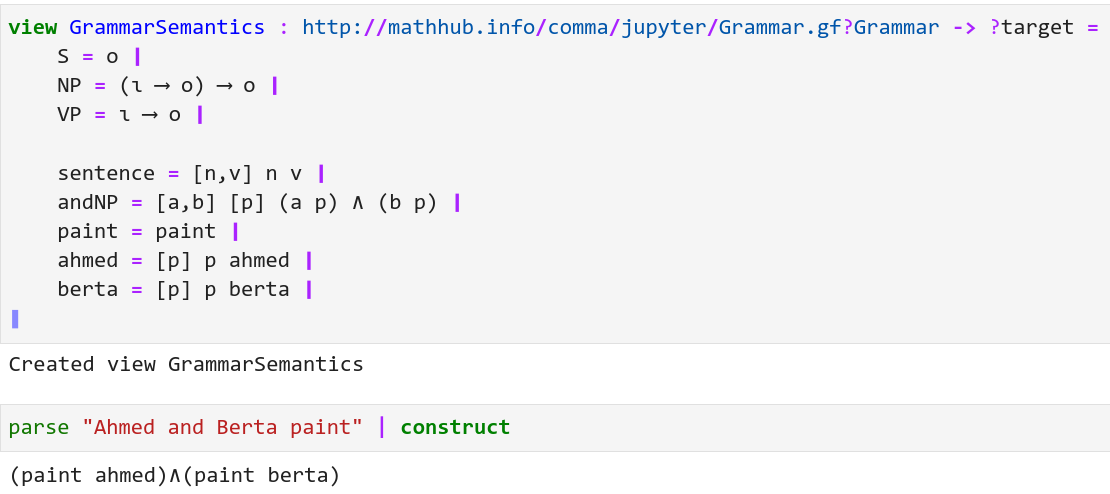
\includegraphics[trim={0 0 20cm 5.7cm},clip,width=0.7\textwidth]{img/screenshot-glif-1.png}}
\end{frame}
}{}

}

% \begin{frame}[fragile]
    \frametitle{Example: Tableaux Machine}
    \begin{itemize}
        \item Can use tableaux for model generation
        \item Tableau machine: pick ``best'' branch as model and continue there with next sentence
            \com{like a human?}
    \end{itemize}

    \vspace{1.5em}
    \begin{minipage}[t][4.5cm]{\textwidth}
        \only<1>{\setshowlevel{1}}
        \only<2>{\setshowlevel{2}}
        \only<3>{\setshowlevel{3}}
        \only<4>{\setshowlevel{4}}
        \includestandalone{fig/tab-machine-simple}
    \end{minipage}
\end{frame}

\begin{frame}
    \frametitle{Example: Tableaux Machine}
    \only<1>{\setshowlevel{1}}
    \only<2>{\setshowlevel{2}}
    \only<3>{\setshowlevel{3}}
    \only<4>{\setshowlevel{4}}
    \makebox[\linewidth]{\includestandalone[scale=0.9]{fig/tab-machine-complex}}
\end{frame}

% 
% \providedisablepart{showscreenshot}
\begin{frame}[fragile]
    \frametitle{Example: Translation}
    \begin{itemize}
        \item Two German words for \str{cousin}, depending on the gender
        \item Two entries in abstract syntax: \verb|cousin_female| and \verb|cousin_male|
        \item Use inference to discard ASTs
    \end{itemize}
    
    \vspace{2em}
    \small
    \begin{minipage}[t][5cm]{\textwidth}
        \begin{tikzpicture}
            \node(eng) at (-4,1) {\parbox{4.2cm}{\str{Kim is Ahmed's cousin and the father of Grace}}};
                \node(ger1) at (-4,-0.5) {\parbox{4.2cm}{\str{Kim ist Ahmeds {\upshape\bf Cousine} und Graces Vater}}};
                \node(ger2) at (-4,-2.0) {\parbox{4.2cm}{\str{Kim ist Ahmeds {\upshape\bf Cousin} und Graces Vater}}};
            \node(ast1) at (0,1) {AST$_1$};
            \node(ast2) at (0,-1) {AST$_2$};
            \only<2->{
                \node(log1) at (3,1) {\color{logicfont} \parbox{2.2cm}{$female(kim) \wedge$ $male(kim)$}};
                \node(log2) at (3,-1) {\color{logicfont} \parbox{2.2cm}{$male(kim) \wedge$ $male(kim)$}};
            }
            \draw[->,thick] (eng) -- (ast1);
            \draw[->,thick] (eng) -- (ast2);
                \draw[->,thick] (ast1) -- (ger1);
                \draw[->,thick] (ast2) -- (ger2);
            \only<2->{
                \draw[->,thick] (ast1) -- (log1);
                \draw[->,thick] (ast2) -- (log2);
            }
            \only<3>{
                \draw[ultra thick,red] (2,1.5) -- (4,0.5);
                \draw[ultra thick,red] (2,0.5) -- (4,1.5);
                
                \draw[ultra thick,red] (-0.5,1.5) -- (0.5,0.5);
                \draw[ultra thick,red] (-0.5,0.5) -- (0.5,1.5);

                \draw[ultra thick,red] (-6,0.0) -- (-2,-1.0);
                \draw[ultra thick,red] (-6,-1.0) -- (-2,0.0);
            }
        \end{tikzpicture}
    \end{minipage}
    \ifpart{showscreenshot}{\only<4>{
        \begin{tikzpicture}[overlay,remember picture]
            \fill[gray!80,opacity=0.8] (current page.north west) rectangle (current page.south east);
            \node at (current page.center) { 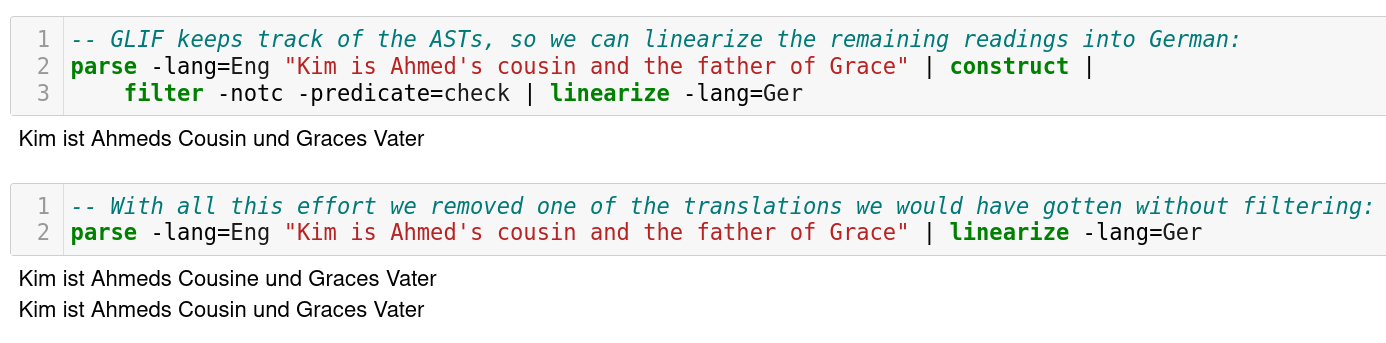
\includegraphics[width=\textwidth]{img/screenshot-glif-5.png} };
        \end{tikzpicture}
    }}{}
\end{frame}

% 
% 
% \begin{frame}
%     \frametitle{GLIF Summary}
%     \includestandalone[width=\textwidth]{fig/glif-architecture}
% \end{frame}
% 
% \begin{frame}
%     \frametitle{Supporting the Semantic/Pragmatic Analysis}
%     Observation:
%     \begin{itemize}
%         \item Parsing and semantics construction are based on specialized frameworks
%         \item ELPI is a more general programming language
%     \end{itemize}
%     
%     \vspace{1em}
%     Can we do something more specialized?
%     \begin{itemize}
%         \item Not really -- there is no ``standard recipe'' for
%             semantic/pragmatic analysis
%         \item But: It usually involves inferential reasoning
%     \end{itemize}
% 
%     \vspace{2em}
%     \centering
%     \bfseries Let's generate provers!\par
% \end{frame}
% 
% \bgroup

% \providecolorgroup{inf}{blue!50!red}
\providecolorgroup{inf}{black}

% used for highlighting parts of the code.
% probably better solutions exist...
\lstset{literate={*1}{\color{hlfont}}{1} {*2}{\color{inffont}}{1} {*3}{\color{inffont!50}}{1}}

\def\proofvdots#1{
    \let\tmpvskip=\extraVskip
    \def\extraVskip{-2pt}
    \noLine
    \UnaryInfC{{$\raisebox{6pt}\vdots$}}
    \noLine
    #1
    \let\extraVskip=\tmpvskip
}
\newcommand\tabdivider{\;\bigl|\;}

\begin{frame}[fragile]
    \frametitle{Natural Deduction in MMT/LF}
    \begin{minipage}{0.9\textwidth}
        \centering
        \begin{minipage}{0.49\textwidth}
            \begin{prooftree}
                \AxiomC{$A \wedge B$}
                \RightLabel{$\wedge El$}
                \UnaryInfC{$A$}
            \end{prooftree}
        \end{minipage}
        \begin{minipage}{0.49\textwidth}
            \begin{prooftree}
                \def\defaultHypSeparation{\hskip 0pt}
                \AxiomC{$A \vee B$}
                \AxiomC{$\,\,[A]^1$}
                \proofvdots{\UnaryInfC{$C$}}
                \AxiomC{$\,\,[B]^1$}
                \proofvdots{\UnaryInfC{$C$}}
                \RightLabel{$\vee E^1$}
                \TrinaryInfC{$C$}
            \end{prooftree}
        \end{minipage}
    \end{minipage}

    \vspace{1.5em}
    \begin{lstlisting}[language=MMT]
    // \vdashX is type of proofs for X (judgments as types)
    \vdash : o \raa type

    \wedgeEl : \PiAo\PiBo \vdashA\wedgeB \raa \vdashA
    \veeE  : \PiAo\PiBo\PiCo \vdashA\veeB \raa (\vdashA \raa \vdashC) \raa (\vdashB \raa \vdashC) \raa \vdashC
    \end{lstlisting}
\end{frame}

\begin{frame}[fragile]
    \frametitle{Generating Provers in ELPI}
%     \begin{itemize}
%         \item ELPI is an extension of $\lambda$Prolog \com{$\approx$ Prolog + HOAS}\note{ELPI was developed by Claudio and others}
%         \item Optimized for fast execution of logical algorithms \com{type inference, unification, proof search, \dots}
%     \end{itemize}
    \makebox[2.5cm][l]{\textbf{LF rule}} \lstinline[language=MMT]|\wedgeEl : \PiAo\PiBo \vdashA\wedgeB \raa \vdashA|

    \vspace{1.0em}
    \textbf{ELPI equivalent}

    \vspace{0.5em}
    \makebox[2.5cm][r]{direct:$\;\;$} \lstinline[language=ELPI]|pi A \ pi B \ ded (and A B) => ded A.|

    \vspace{0.5em}
    \makebox[2.5cm][r]{syn. sugar:$\;\;$} \lstinline[language=ELPI]|ded A :- ded (and A B).|

% \end{frame}
% 
% \begin{frame}[fragile]
%     \frametitle{From LF to ELPI}
    % \textbf{Or-elimination}
    \vspace{1.5em}
    \pause

    \begin{block}{{\bfseries Example:} Or-Elimination}
    \makebox[1.2cm][l]{LF:}\begin{minipage}{0.85\textwidth}
        \lstinline[keepspaces=true,language=MMT]|\veeE : \PiAo\PiBo\PiCo \vdashA\veeB \raa (\vdashA \raa \vdashC) \raa (\vdashB \raa \vdashC) \raa \vdashC|
    \end{minipage}

    \vspace{0.5em}
    \makebox[1.2cm][l]{ELPI:}\lstinline[language=ELPI,keepspaces=true]|ded C :- ded (or A B), ded A => ded C, ded B => ded C.|
    \end{block}

    \vspace{0.5em}

    \begin{block}{{\bfseries Example:} Forall-Introduction}
    % \textbf{Forall-introduction}
    \makebox[1.2cm][l]{LF:}\begin{minipage}{0.85\textwidth}
        \lstinline[keepspaces=true,language=MMT]|\forallI : \PiPio (\Pixi \vdashP x) \raa \vdash\forallP|
    \end{minipage}

    \vspace{0.5em}
    \makebox[1.2cm][l]{ELPI:}\lstinline[language=ELPI,keepspaces=true]|ded (forall P) :- pi x \ ded (P x).|
    \vspace{0.5em}
    \end{block}
\end{frame}

\begin{frame}[fragile]
    \frametitle{Controlling the Proof Search}
    \begin{itemize}
        \item Problem: Search diverges \com{searching harder than checking}
        \item Solution: Control search with helper predicates:
            \com{inspired by ProofCert project by Miller et al.}\note{ProofCert assumes a focused logic, we don't}
            % \\{ \itshape\color{black!50}\makebox[10cm][r]{(inspired by ProofCert project by Miller et al.)}}
            \begin{itemize}
                \item Intuition: Decide whether to apply rule
                \item Do not affect correctness
                \item Extra argument tracks aspects of proof state
            \end{itemize}
    \end{itemize}

    \vspace{1.5em}
    \makebox[1.2cm][l]{Before:}{{
    \lstinline[language=ELPI,keepspaces=true]|ded*1 *2A :-*1                      *2ded *1   *2(and A B).|
    }}

    \vspace{0.5em}
    \makebox[1.2cm][l]{Now:}{{
    \lstinline[language=ELPI,keepspaces=true]|ded*1X*2A :- *1help/andEl X A B X1, *2ded *1X1 *2(and A B).|
    }}

%     \vspace{2.0em}
%     Example helper for depth-limit:
% 
%     \vspace{0.5em}
%     \lstinline[language=ELPI,keepspaces=true]|    help/andEl (idcert N) _ _ (idcert N1) :- N > 0, N1 is N - 1.|
\end{frame}

\begin{frame}[fragile]
    \frametitle{Helper Predicates}
        \renewcommand{\arraystretch}{1.5}
    \begin{tabular}{l p{4cm} p{4.5cm}}
        \textbf{Name} & \textbf{Predicate} & \textbf{Argument} \\
        Iter. deepening & checks depth & remaining depth \\
        Proof term & generates term & proof term \\
        Product & calls other predicates & arguments for other predicates \\
        Backchaining &
            \footnotesize Prolog's backchaining ($\approx$ forward reasoning from axioms via $\Rightarrow$/$\forall$ elimination rules) &
            \footnotesize pattern of formula to be proven (e.g. a conjunction) \\
        % Backchaining & \multicolumn2{p{7cm}}{\footnotesize Restricts new formulae in e.g. elimination rules to those that could be proven by forward reasoning} \\
    \end{tabular}

    \vspace{1.5em}
    \begin{block}{\textbf{Example helper:} Iterative deepening}
        \lstinline[language=ELPI,keepspaces=true]|help/andEl (idcert N) _ _ (idcert N1) :- N > 0, N1 is N - 1.|
    \end{block}

%     Example call:
%     \begin{lstlisting}[language=ELPI]
%     ?- ded (prodcert (idcert 2) (ptcert Proof)) (impl a (or a b)).
% 
%     Proof = implI a (or a b) (orIl a b (i a)).
%     \end{lstlisting}
\end{frame}

\begin{frame}[fragile]
    \frametitle{Tableau Provers}
    \note{We can scale in terms of logics supported or (orthogonally) in terms of prover strategies.
    We went for the latter.}
    \begin{minipage}[b][2cm][b]{0.4\textwidth}
        \begin{prooftree}
            \AxiomC{$\;\tabfalse{A \wedge B}$}
            \RightLabel{$\tabfalse\wedge$}
            \UnaryInfC{$\tabfalse{A} \tabdivider \tabfalse{B}$}
        \end{prooftree}
    \end{minipage}
    \begin{minipage}[b][2cm][b]{0.4\textwidth}
        \def\defaultHypSeparation{\hskip 0pt}
        \begin{prooftree}
            \AxiomC{$\tabfalse{A \wedge B}$}
            \AxiomC{$\;[\tabfalse{A}]$}
            \proofvdots{\UnaryInfC{$\bot$}}
            \AxiomC{$\;[\tabfalse{B}]$}
            \proofvdots{\UnaryInfC{$\bot$}}
            \RightLabel{$\tabfalse\wedge$}
            \TrinaryInfC{$\bot$}
        \end{prooftree}
    \end{minipage}

    \vspace{2em}
    \makebox[1.0cm][l]{LF:} \lstinline[language=MMT]|\wedge\tabfalse : \PiAo\PiBo A\wedgeB\tabfalse \raa (A\tabfalse \raa \bot) \raa (B\tabfalse \raa \bot) \raa \bot|

    \vspace{0.5em}
    \makebox[1.0cm][l]{ELPI:} \lstinline[language=ELPI]|closed *3X *2:- *3help/andF X A B X1 X2 X3, *2f *3X1 *2(and A B),|
    \lstinline[language=ELPI,keepspaces=true]|                         f*3/hyp *2A => closed *3X2*2, f*3/hyp*2 B => closed *3X3*2.|

    \vspace{2em}
    With iterative deepening we get a working prover!

    $\rightarrow$ Other helpers result in more efficient provers
\end{frame}

\egroup

% 
% \begin{frame}
%     \frametitle{Conclusion: Prototyping NLU Pipelines}
%     \includestandalone[width=\textwidth]{fig/glif-spec}
% \end{frame}

\appendix

\begin{frame}[allowframebreaks,t]
    \frametitle{References}
    \printbibliography
\end{frame}

\end{document}
